\section{Detector response and responsivity}
\label{sec:theory.response}

In the quasiparticle number model, the response of a KID to light is determined by the following chain of relations.
First, the optical power absorbed by the detector is the product of the incident power and the optical efficiency.
Second, the absorbed power, photon energy, and material parameters determine the optical quasiparticle generation rate.
Third, the total quasiparticle generation rate and the various quasiparticle decay channels determine the quasiparticle number.
Fourth, the quasiparticle number determines the complex conductivity.
Fifth, the complex conductivity and resonator geometry determine the surface impedance.
Sixth, the surface impedance and resonator geometry determine the resonance frequency and quality factors of the resonator.
Seventh, the resonator parameters and readout tone frequency determine the forward scattering parameter that is measured by the readout electronics.
This is a long list, but most of these relationships turn out to be simple.
I use \textit{response} to mean the shift in some quantity from the zero-illumination case and use \textit{responsivity} to mean the derivative at a particular operation point.


\subsection{Photodetection}
\label{sec:theory.response.photodetection}

If the incident optical power at some reference plane is $\power_\incident$ and the optical power absorbed in the active region of the detector is $\power_\optical$, then the optical efficiency $\efficiency_\incident$ for power at this plane relates them:
\begin{equation}
\label{eqn:photodetection.response}
\power_\optical = \efficiency_\incident \power_\incident.
\end{equation}
The responsivity is
\begin{equation}
\label{eqn:photodetection.responsivity}
\pdv{\power_\optical}{\power_\incident}
  =
  \efficiency_\incident.
\end{equation}
The process by which the absorption occurs depends on the detector architecture.
In the lumped-element KIDs discussed in Chapters~\ref{chp:loss} and \ref{chp:sensitivity}, millimeter-wave light is concentrated by a feed horn onto a meandering inductor that forms the sensing region of the detector.
For the co-planar waveguide KIDs discussed in Chapter~\ref{chp:multichroic}, the light is coupled through a feedhorn into a planar ortho-mode transducer (OMT) antenna, and routed through millimeter-wave circuitry into the high-current (shorted) end of a quarter-wave CPW resonator.
\todo[inline]{Discuss conductivity just above cutoff}
\begin{comment}
For frequencies $\foptical$ more than a few times the optical cutoff frequency $\foptical_\cutoff = 2 \gap / \planck$,
$\reconductivity(\foptical) = \normalconductivity$
and
$\imconductivity(\foptical) = 0$.
For frequencies closer to the gap, the Mattis-Bardeen equations should be used to obtain more accurate results.
\end{comment}
Chapter~\ref{chp:sensitivity} discusses a method for obtaining the optical efficiency, and thus the absorbed power, from measurements of the noise level.
\todo[inline]{Plot $\conductivity$ for $\foptical > \foptical_\cutoff$ and discuss.}
\todo[inline]{Discuss LEKID impedance matching.}
\todo[inline]{Any difference between A normal to film and A in plane?}
\todo[inline]{Discuss Popel exact thin-film solution}


\begin{figure}[htb]
\centering
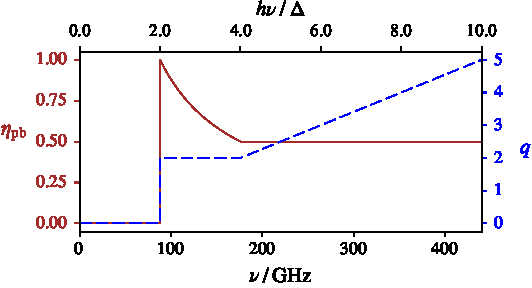
\includegraphics[width=0.9\textwidth]{theory/quasiparticles_per_photon_and_pairbreaking_efficiency.pdf}
\caption
[The number of quasiparticles excited per photon and the pair-breaking efficiency versus photon frequency.]
{A sketch of the number of quasiparticles excited per photon and the pair-breaking efficiency, both plotted versus photon frequency and photon energy in units of the gap.
The values on the upper horizontal axis are universal, while the frequency values on the lower horizontal axis are calculated for a BCS superconductor with the bulk aluminum $\tc = \SI{1.2}{K}$.
For $\planck \foptical > 4 \gap$, the phonon trapping factor $\phonontrapping$ affects the fraction of photon energy that is converted into quasiparticles.
Figure~4 of \textcite{Guruswamy2014SUST} shows a theoretical calculation of $\pbefficiency$ that suggests $0.4 < \pbefficiency < 0.6$ at higher energies.
The choice made here of $\pbefficiency = 0.5$ corresponds to a phonon trapping factor $\phonontrapping \sim 3$.
Figure~2 of \textcite{deVisser2015APL} shows a measurement of $\pbefficiency$ that qualitatively agrees with this figure.
\todo[inline]{Re-create this pair-breaking plot with harmonized fiducials.}}
\label{fig:quasiparticles_per_photon_and_pairbreaking_efficiency}
\end{figure}

\subsection{Optical quasiparticle generation}
\label{sec:theory.response.generation}

As the optical power $\power_\optical$ is absorbed in the active region of the KID, each absorbed photon generates $\qpperphoton \ge 2$ quasiparticles on average.
The number of quasiparticles excited by a given photon with $\planck \foptical \ge 4 \gap$ may vary, and for very high-energy photons the details of the down-conversion process are complex~\autocite{Kozorezov2000PRB}.
For KIDs designed to resolve the energy of single photons, the variation of the created quasiparticle number is a fundamental source of noise~\autocite{Mazin2005}.
However, this variation is not important for photometric detectors, which do not resolve individual photon arrivals.
The variance of the quasiparticle number under steady illumination will turn out to be linear in $\qpperphoton$, so we can obtain correct results for the noise while considering only the average number of excitations per photon.
Most of the measurements presented here are made using photon energies $\planck \foptical \gtrsim 2 \gap$, where $\qpperphoton = 2$ exactly.

In the KID literature one often encounters the pair-breaking efficiency
\begin{equation}
\pbefficiency
  =
  \frac{\qpperphoton \expval{\energy_\quasiparticle}}{\planck \foptical}
  \approx
  \frac{\qpperphoton \gap}{\planck \foptical},
\label{eqn:pbefficiency}
\end{equation}
where $\expval{\energy_\quasiparticle} \gtrsim \gap$ is the average quasiparticle energy.
Approximately, $\pbefficiency$ is the fraction of photon energy that is converted into energy in the steady-state quasiparticle system.
Figure~\ref{fig:quasiparticles_per_photon_and_pairbreaking_efficiency} is a sketch of $\qpperphoton$ and $\pbefficiency$ for photon energies $\planck \foptical$ near the spectroscopic gap.
For $\planck \foptical < 2 \gap$, no quasiparticles are excited because the excitations must be created in pairs.
For $2 \gap < \planck \foptical < 4 \gap$, each photon excites exactly two quasiparticles and the remaining energy is converted into phonons that do not have sufficient energy to break additional pairs.
For $4 \gap < \planck \foptical$ each photon may break more than one pair, and approximately half the photon energy is converted into quasiparticles.
The value $\pbefficiency \approx 0.6$ is commonly used.
However, as discussed in detail by \textcite{Guruswamy2014SUST}, $\pbefficiency$ depends on the details of phonon trapping: it is lower when the phonon trapping factor is lower because a high-energy phonon is more likely to escape before depositing its energy in the quasiparticle system.

Thus, if a detector absorbs optical power $\power_\optical$ from photons with frequency $\foptical$, the optical quasiparticle generation rate is
\begin{equation}
\Rate_\optical
  =
  \frac{\qpperphoton \power_\optical}{\planck \foptical}
  =
  \frac{\pbefficiency \power_\optical}{\gap},
\label{eqn:optical_generation.response}
\end{equation}
and the responsivity is
\begin{equation}
\pdv{\Rate_\optical}{\power_\optical}
  =
  \frac{\qpperphoton}{\planck \foptical}
  =
  \frac{\pbefficiency}{\gap}.
\label{eqn:optical_generation.responsivity}
\end{equation}


\subsection{Quasiparticle number}
\label{sec:theory.response.qpnumber}

It is difficult to uniformly illuminate the active (sensing) region of a KID, so the generation rate is likely to vary with position.
Nevertheless, we now assume that diffusion  equalizes the quasiparticle density within the active region of the resonator.
This allows us to use the results of Section~\ref{sec:theory.qpnumber} with the quasiparticle density replaced by the quasiparticle number
$\qpnumber = \volume \qpdensity$,
where $\volume$ is the active volume.
The quasiparticle number depends on the total generation rate
$\Rate_\generation = \rate_\generation \volume$,
which accounts for all generation sources, such as absorption of optical photons, readout photons, and thermal phonons:
\begin{equation}
\Rate_\generation
  =
  \Rate_\optical + \Rate_\readout + \Rate_\thermal.
\end{equation}
We expect these rates to be approximately independent so that
$
\pdv*{\qpnumber}{\Rate_\optical}
  =
  \pdv*{\qpnumber}{\Rate_\generation}.
$

The steady-state quasiparticle number is given by Equation~\ref{eqn:ssqpdensity} multiplied by $\volume$:
\begin{equation}
\ssqpnumber
  = 
  \left( \left(\frac{\volume \qpsingledecay}{2 \qprecombinationeff}\right)^2
  + \frac{\volume \ssRate_\generation}{\qprecombinationeff} \right)^{1/2}
  - \frac{\volume \qpsingledecay}{2 \qprecombinationeff},
\label{eqn:qpnumber.response}
\end{equation}
with
$\ssqpnumber = (\volume \ssRate_\generation / \qprecombinationeff)^{1/2}$
when single-quasiparticle decay is negligible.

The corresponding responsivity to slow perturbations around this number is given by Equation~\ref{eqn:qprelaxationtime}:
\begin{equation}
\pdv{\ssqpnumber}{\ssRate_\generation}
  =
  \qprelaxationtime
  =
  \left( \frac{2 \qprecombinationeff \ssqpnumber}{\volume} + \qpsingledecay \right)^{-1}
  =
  \left( \frac{2 \ssRate_\generation}{\ssqpnumber} - \qpsingledecay \right)^{-1}
  =
  \left( \frac{4 \qprecombinationeff \ssRate_\generation}{\volume} + \qpsingledecay^2 \right)^{-1/2}.
\label{eqn:qpnumber.responsivity}
\end{equation}
This equation is valid only for perturbations that occur on time scales much larger than $\qprelaxationtime$.
To describe faster perturbations, we may define
$\delta\qpnumber(\time) = \qpnumber(\time) - \ssqpnumber$
and 
$\delta\Rate_\generation(\time) = \Rate_\generation(\time) - \ssRate_\generation$, and the corresponding Fourier transforms
\begin{equation}
\delta\qpnumber(\time)
  =
  \int_{-\infty}^\infty \dd{\faudio}
  \exp(2 \pi \I \faudio \time) \, \delta\qpnumber(\faudio)
  \qqtext{and}
\delta\Rate_\generation(\time)
  =
  \int_{-\infty}^\infty \dd{\faudio}
  \exp(2 \pi \I \faudio \time) \, \delta\Rate_\generation(\faudio).
\end{equation}
The solution is just Equation~\ref{eqn:delta_qpdensity_frequency} multiplied by the active volume $\volume$:
\begin{equation}
\delta\qpnumber(\faudio)
  =
  \frac{\qprelaxationtime}{1 + 2 \pi \I \faudio \qprelaxationtime} \delta\Rate_\generation(\faudio).
\label{eqn:delta_qpnumber_frequency}
\end{equation}
As shown above, the optical generation rate $\Rate_\optical$ is proportional to the absorbed optical power $\power_\optical$;
as shown below, the quantities measured by the KID readout system are proportional to $\qpnumber$.
Thus, when optical generation dominates, we expect the detector response to go as $\power_\optical^{1/2}$ and the responsivity to go as $\power_\optical^{-1/2}$.
The data shown in Figure~\ref{fig:measuring.results} behave according to this prediction.


\subsection{Complex conductivity}
\label{sec:theory.response.complex_conductivity}

The complex conductivity $\conductivity$ for an arbitrary quasiparticle occupancy $\qpoccupancy(\energy)$ is determined by the Mattis-Bardeen equations, given in Section~\ref{sec:theory.electrodynamics.mattis-bardeen}.
KIDs should be operated at
$\temperature \ll \tc$
and should be designed so that, under the highest expected illumination, both real and imaginary parts of the change in the complex conductivity remain small compared to the zero temperature value:
\begin{equation}
\frac{\conductivity - \conductivity(0)}{\imconductivity(0)}
  =
  \frac{\braket*{\responseqpoccupancy_{\reconductivity}}{\qpoccupancy} - \I \braket*{\responseqpoccupancy_{\imconductivity}}{\qpoccupancy}}{\imconductivity(0)},
\end{equation}
where
$\imconductivity(0)
  =
  \pi \gap_\zerotemp \normalconductivity / \planck \freadout$.
To use analytic results for the conductivity response, I will assume that $\qpoccupancy$ remains sufficiently small that the first-order approximations discussed in Section~\ref{sec:theory.perturbation} and Appendix~\ref{chp:first-order_response} remain accurate.
As shown by Figures~\ref{fig:responseqpoccupancy_conductivity_f_mc} and~\ref{fig:responseqpoccupancy_conductivity_f_1p}, the response functions for the components of the conductivity are quite different, so an arbitrary perturbation to the occupancy could cause unrelated shifts in $\reconductivity$ and $\imconductivity$.
We avoid this complication using the assumption, also introduced in Section~\ref{sec:theory.perturbation},
that perturbations $\delta\qpoccupancy$ are proportional to $\ssqpoccupancy$.
In this case, the responsivity is 
\begin{equation}
\frac{\delta\conductivity}{\delta\qpnumber}
  =
  \frac{\braket*{\responseqpoccupancy_{\conductivity}}{\delta\qpoccupancy}}{\braket*{\responseqpoccupancy_{\qpnumber}}{\delta\qpoccupancy}}
  =
  \frac{\braket*{\responseqpoccupancy_{\conductivity}}{\ssqpoccupancy}}{\braket*{\responseqpoccupancy_{\qpnumber}}{\ssqpoccupancy}}
  =
  \frac{\conductivity - \conductivity(0)}{\qpnumber}.
\end{equation}
Taking real and imaginary parts gives
\begin{equation}
\frac{\delta\reconductivity}{\delta\qpnumber}
  =
  \frac{\braket*{\responseqpoccupancy_{\reconductivity}}{\ssqpoccupancy}}{\braket*{\responseqpoccupancy_{\qpnumber}}{\ssqpoccupancy}}
\qqtext{and}
\frac{\delta\imconductivity}{\delta\qpnumber}
  =
\frac{\braket*{\responseqpoccupancy_{\imconductivity}}{\ssqpoccupancy}}{\braket*{\responseqpoccupancy_{\qpnumber}}{\ssqpoccupancy}}.
\label{eqn:delta_conductivity_delta_qpnumber}
\end{equation}
When the quasiparticle number increases, the real part of the conductivity increases and the imaginary part decreases.

\begin{figure}[htb]
\centering
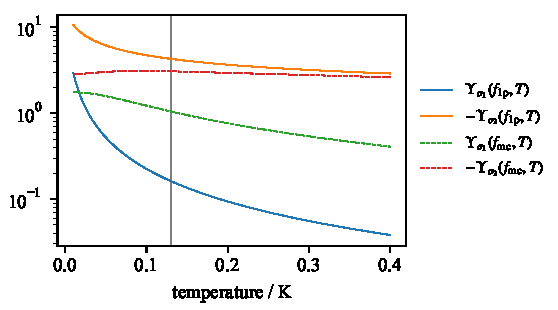
\includegraphics[width=0.8\textwidth]{theory/normresponse_conductivity_thermal.pdf}
\caption[The normalized response ratios of the real and imaginary conductivity to the thermal quasiparticle density.]
{
The normalized response ratios of the real and imaginary conductivity to the thermal quasiparticle density.
The vertical gray line marks the fiducial bath temperature, assuming fiducial values for aluminum.
}
\label{fig:normresponse_conductivity_thermal}
\end{figure}

We can express the ratios of the real and imaginary components of the conductivity response to the quasiparticle density response in dimensionless form (using the same normalization constants, up to a sign, as \textcite{Zmuidzinas2012ARCMP}):
\begin{align}
\begin{split}
\normresponse_{\reconductivity}[\qpoccupancy]
  &=
  \frac{\braket*{\responseqpoccupancy_{\reconductivity}}{\qpoccupancy} / \imconductivity(0)}{\braket*{\responseqpoccupancy_{\qpdensity}}{\qpoccupancy} / 2 \ssdos \gap_\zerotemp}; \\
\normresponse_{\imconductivity}[\qpoccupancy]
  &=
  \frac{\braket*{\responseqpoccupancy_{\imconductivity}}{\qpoccupancy} / \imconductivity(0)}{\braket*{\responseqpoccupancy_{\qpdensity}}{\qpoccupancy} / 2 \ssdos \gap_\zerotemp}.
\end{split}
\label{eqn:normresponse_conductivity}
\end{align}
These functions must be calculated numerically for an arbitrary occupancy.
For a thermal occupancy we can use Equations~\ref{eqn:qpdensity_thermal}, \ref{eqn:responseqpoccupancy_reconductivity_thermal}, and \ref{eqn:responseqpoccupancy_imconductivity_thermal} to obtain
\begin{equation}
\normresponse_{\reconductivity}(\temperature)
  =
  \left( \frac{8 \gap_\zerotemp}{\pi^3 \kb \temperature} \right)^{1/2}
  \sinh \left( \frac{\planck \freadout}{2 \kb \temperature} \right)
  K_0 \left( \frac{\planck \freadout}{2 \kb \temperature} \right)
\label{eqn:normresponse_reconductivity_thermal}
\end{equation}
and
\begin{equation}
\normresponse_{\imconductivity}(\temperature)
  =
  - \left[
  1 + \left( \frac{2 \gap_\zerotemp}{\pi \kb \temperature} \right)^{1/2}
  \exp \left( -\frac{\planck \freadout}{2 \kb \temperature} \right)
  I_0 \left( \frac{\planck \freadout}{2 \kb \temperature} \right)
  \right].
\label{eqn:normresponse_imconductivity_thermal}
\end{equation}
These functions are plotted in Figure~\ref{fig:normresponse_conductivity_thermal} for the fiducial readout frequencies.
The imaginary part of the conductivity responds much more to quasiparticles than the real part.
Additionally, at the fiducial bath temperature, the ratio of the reactive response to the dissipative response
$\jonasbeta(\temperature, \freadout)
  \equiv
  |\normresponse_{\imconductivity}(\temperature, \freadout) / \normresponse_{\reconductivity}(\temperature, \freadout)|$
is nearly 30 at $\freadout_\singlepol$, while it is only about 3 at $\freadout_\multichroic$.
These predictions will turn out to be approximately true even under optical illumination.

Finally, combining Equation~\ref{eqn:delta_conductivity_delta_qpnumber} with Equation~\ref{eqn:normresponse_conductivity} gives
\begin{equation}
\pdv{\reconductivity}{\qpnumber}
  =
  \frac{\imconductivity(0)}{2 \ssdos \gap_\zerotemp \volume} \normresponse_{\reconductivity}[\qpoccupancy]
\label{eqn:delta_reconductivity_delta_qpnumber_normresponse}
\end{equation}
and
\begin{equation}
\pdv{\imconductivity}{\qpnumber}
  =
  \frac{\imconductivity(0)}{2 \ssdos \gap_\zerotemp \volume} \normresponse_{\imconductivity}[\qpoccupancy].
\label{eqn:delta_imconductivity_delta_qpnumber_normresponse}
\end{equation}
Because $\normresponse_{\imconductivity}$ is negative, the imaginary part of the complex conductivity decreases with increasing quasiparticle number.


\subsection{Surface impedance}
\label{sec:theory.response.surface_impedance}

Taking derivatives of the first-order expressions in Equation~\ref{eqn:surface_resistance_and_reactance_shift} leads to
\begin{equation}
\pdv{\resistance_\surface}{\reconductivity}
  =
  \frac{\surfimpexp \reactance_\surface(0)}{\imconductivity(0)},
\end{equation}
and
\begin{equation}
\pdv{\reactance_\surface}{\imconductivity}
  =
  - \frac{\surfimpexp \reactance_\surface(0)}{\imconductivity(0)}.
\end{equation}


\subsection{Resonator parameters}
\label{sec:theory.response.resonator}

From Section~\ref{sec:theory.resonator}, we have
\begin{equation}
\loss_\quasiparticle
  =
  \frac{\kifraction \resistance_\surface}{\reactance_\surface(0)}
\end{equation}
and
\begin{equation}
\shift
  =
  \frac{\kifraction}{2} \frac{\reactance_\surface - \reactance_\surface(0)}{\reactance_\surface(0)}.
\end{equation}
The responsivities are thus
\begin{equation}
\pdv{\loss_\quasiparticle}{\resistance_\surface}
  =
  \frac{\kifraction}{\reactance_\surface(0)}
\label{eqn:delta_loss_internal_delta_resistance_surface}
\end{equation}
and
\begin{equation}
\pdv{\detuning}{\reactance_\surface}
  =
  \pdv{\shift}{\reactance_\surface}
  =
  \frac{\kifraction}{2 \reactance_\surface(0)}.
\label{eqn:delta_detuning_delta_reactance_surface}
\end{equation}


\begin{figure}[htb]
\centering
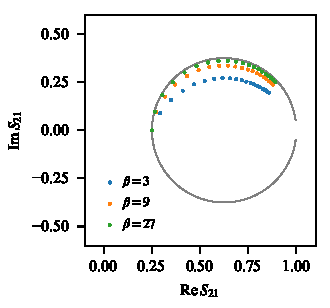
\includegraphics[width=0.8\textwidth]{theory/s21_response.pdf}
\caption
[Theoretical predictions for the $\forwardscattering$ response to an increase in the quasiparticle number.]
{
Theoretical predictions for the $\forwardscattering$ response to an increase in the quasiparticle number.
The parameter
$\jonasbeta
  =
  - \normresponse_{\imconductivity} / \normresponse_{\reconductivity}
  =
  2 \delta\detuning / \delta\loss_\internal$
determines the trajectory of the response in the complex $\forwardscattering$ plane.
}
\label{fig:s21_response}
\end{figure}

\subsection{The forward scattering parameter}
\label{sec:theory.response.forwardscattering}

\todo[inline]{Move this content to the resonator section}
When the resonator parameters $\loss_\internal(\time)$ and $\detuning(\time)$ change slowly, the $\forwardscattering$ response is given by the partial derivatives in the obvious way:
\begin{equation}
\adiabatici
  \equiv
  \pdv{\forwardscattering}{\loss_\internal}
  =
  \frac{(1 + \I \asymmetry) \loss_\coupling}{(\loss_\coupling + \loss_\internal + 2 \I \detuning)^2}
  =
  \frac{(1 - \forwardscattering)^2}{(1 + \I \asymmetry) \loss_\coupling}
\end{equation}
and
\begin{equation}
\adiabaticx
  \equiv
  \pdv{\forwardscattering}{\detuning} 
  =
  2 \I \pdv{\forwardscattering}{\loss_\internal}
  =
    \frac{(2 \I - 2 \asymmetry) \loss_\coupling}{(\loss_\coupling + \loss_\internal + 2 \I \detuning)^2}
  =
  \frac{2 \I (1 - \forwardscattering)^2}{(1 + \I \asymmetry) \loss_\coupling}.
\end{equation}
Factoring these equations shows that the response is maximized when $\detuning = 0$ and when $\loss_\internal = \loss_\coupling$~\autocite{Zmuidzinas2012ARCMP}.
When $\detuning = 0$ and $\asymmetry = 0$, $\forwardscattering$  and $\adiabatici$ are purely real, while $\adiabaticx$ is purely imaginary.
The partial derivatives are orthogonal even when these conditions are not satisfied, and they correspond to directions that are tangent to and normal to the resonance circle.

The forward scattering parameter does not react instantly to changes in the resonator parameters, and this effect can be accounted for using a resonator transfer function $\restransfer$.
When $\detuning = 0$, the Fourier domain transfer function is just a single-pole low-pass filter with the same shape as the resonator~\autocite{Gao2008,Zmuidzinas2012ARCMP}:
$\restransfer(\faudio)
  =
  \left( 1 + \I \faudio / \faudio_\resonator \right)^{-1}$,
where $\faudio$ is the signal frequency and
$\faudio_\resonator = \freadout_\resonator \loss_\resonator / 2$
is the resonator bandwidth, which is half its linewidth.
The resonator bandwidth is generally much larger than the quasiparticle bandwidth.
However, the lumped-element resonators discussed in Chapters~\ref{chp:loss}~and~\ref{chp:sensitivity} have unusually low resonance frequencies and low internal loss, and for these resonators the two bandwidths are similar.


\subsection{Summary}
\label{sec:theory.response.summary}

\begin{figure}[htb]
\centering
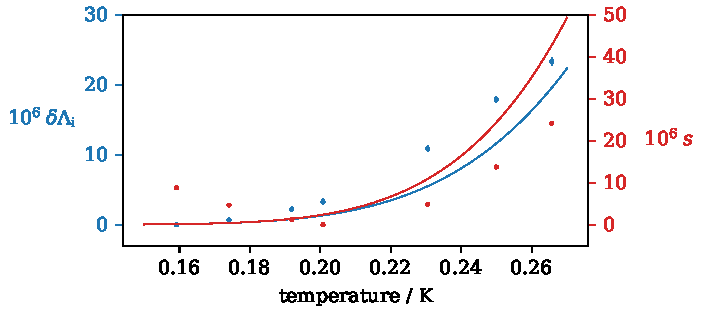
\includegraphics[width=\textwidth]{theory/mkidarray02_chosen_one_di_and_s_versus_temperature.pdf}
\caption[MKIDArray02-0001: the internal loss and fractional frequency shift versus temperature for a multichroic \SI{3410}{MHz} resonator.]
{
MKIDArray02-0001: the change in internal loss and fractional frequency shift versus temperature for a multichroic \SI{3410}{MHz} resonator.
Here,
$\delta\loss_\internal = \loss_\internal - \loss_\internal^\mathrm{min}$.
The points are the measured data, and the corresponding lines are Equation~\ref{eqn:ssloss_quasiparticle} for the internal loss and Equation~\ref{eqn:ssshift} for the fractional frequency shift, both evaluated using fiducial parameters and an effective kinetic inductance fraction $\kifraction = 0.2$.
}
\label{fig:mkidarray02_chosen_one_di_and_s_versus_temperature}
\end{figure}

We can now combine equations from the preceding sections to obtain the detector response and responsivity.
The steady-state quasiparticle loss is
\begin{equation}
\ssloss_\quasiparticle
  =
  \frac{\kifraction}{\reactance_\surface(0)}
  \frac{\surfimpexp \reactance_\surface(0)}{\imconductivity(0)}
  \ssreconductivity
  =
  \frac{\kifraction \surfimpexp}{\imconductivity(0)}
  \braket*{\responseqpoccupancy_{\reconductivity}}{\ssqpoccupancy},
\label{eqn:ssloss_quasiparticle}
\end{equation}
and the steady-state fractional frequency shift is
\begin{equation}
\ssshift
  =
  \frac{\kifraction}{2 \reactance_\surface(0)}
  \left( -\frac{\surfimpexp \reactance_\surface(0)}{\imconductivity(0)} \right)
  \left[ \ssimconductivity - \imconductivity(0) \right]
  =
  -\frac{\kifraction \surfimpexp}{2 \imconductivity(0)}
  \braket*{\responseqpoccupancy_{\imconductivity}}{\ssqpoccupancy}.
\label{eqn:ssshift}
\end{equation}
(Recall that $\responseqpoccupancy_{\imconductivity}$ is negative.)
Figure~\ref{fig:mkidarray02_chosen_one_di_and_s_versus_temperature} shows the above equations, calculated for a thermal occupancy, along with data from a multichroic CPW KID.
The theory and data agree within about a factor of two, but the behavior of this resonator appears to be significantly affected by two-level systems in nearby dielectrics.
(See Section~\ref{sec:loss.dielectrics} and Section~\ref{sec:multichroic.mkidarray02}.)

To describe time-dependent perturbations around these values, caused by $\delta\qpoccupancy(\time)$, we can write
\begin{align}
\begin{split}
\delta\loss_\quasiparticle(\time)
  =
  \pdv{\loss_\quasiparticle}{\resistance_\surface}
  \pdv{\resistance_\surface}{\reconductivity}
  \delta\reconductivity(\time)
  &=
  \frac{\kifraction \surfimpexp}{\imconductivity(0)}
  \braket*{\responseqpoccupancy_{\reconductivity}}{\delta\qpoccupancy(\time)} \\
  &=
  \frac{\kifraction \surfimpexp}{\imconductivity(0)}
  \frac
  {\braket*{\responseqpoccupancy_{\reconductivity}}{\ssqpoccupancy}}
  {\braket*{\responseqpoccupancy_{\qpnumber}}{\ssqpoccupancy}}
  \braket*{\responseqpoccupancy_{\qpnumber}}{\delta\qpoccupancy(\time)} \\
  &=
  \frac{\kifraction \surfimpexp \ssnormresponse_{\reconductivity}}{2 \ssdos \gap_\zerotemp \volume} \delta\qpnumber(\time),
\end{split}
\end{align}
where $\ssnormresponse_{\reconductivity} = \normresponse_{\reconductivity}[\ssqpoccupancy]$, and
\begin{align}
\begin{split}
\delta\detuning(\time)
  =
  \pdv{\detuning}{\reactance_\surface}
  \pdv{\reactance_\surface}{\imconductivity}
  \delta\imconductivity(\time)
  &=
  -\frac{\kifraction \surfimpexp}{2 \imconductivity(0)}
  \braket*{\responseqpoccupancy_{\imconductivity}}{\delta\qpoccupancy(\time)} \\
  &=
  -\frac{\kifraction \surfimpexp}{2 \imconductivity(0)}
  \frac
  {\braket*{\responseqpoccupancy_{\imconductivity}}{\ssqpoccupancy}}
  {\braket*{\responseqpoccupancy_{\qpnumber}}{\ssqpoccupancy}}
  \braket*{\responseqpoccupancy_{\qpnumber}}{\delta\qpoccupancy(\time)} \\
  &=
  -\frac{\kifraction \surfimpexp \ssnormresponse_{\imconductivity}}{4 \ssdos \gap_\zerotemp \volume} \delta\qpnumber(\time),
\end{split}
\end{align}
where
$\ssnormresponse_{\imconductivity} = \normresponse_{\imconductivity}[\ssqpoccupancy]$
and 
$\delta\imconductivity = \imconductivity - \ssimconductivity$.
Since $\normresponse_{\imconductivity}$ is negative, both $\delta\loss_\internal$ and $\delta\detuning$ increase when the quasiparticle number increases.
Finally, we can relate the quasiparticle number to the generation rate, which is proportional to the absorbed power.
The steady-state values will be set by the steady-state generation rate $\ssRate_\generation$.
As above, consider small perturbations
$\delta\Rate_\generation(\time)
  =
  \Rate_\generation(\time) - \ssRate_\generation$ around this rate.
Then, given the frequency-domain perturbation $\delta\Rate_\generation(\faudio)$, the frequency-domain quasiparticle loss response is
\begin{equation}
\delta\loss_\quasiparticle(\faudio)
  =
  \frac{\kifraction \surfimpexp \ssnormresponse_{\reconductivity}}{2 \ssdos \gap_\zerotemp \volume}
  \frac{\qprelaxationtime}{1 + 2 \pi \I \faudio \qprelaxationtime}
  \delta\Rate_\generation(\faudio).
\end{equation}
Similarly, the frequency-domain detuning response is
\begin{equation}
\delta\detuning(\faudio)
  =
  -\frac{\kifraction \surfimpexp \ssnormresponse_{\imconductivity}}{4 \ssdos \gap_\zerotemp \volume}
  \frac{\qprelaxationtime}{1 + 2 \pi \I \faudio \qprelaxationtime}
  \delta\Rate_\generation(\faudio).
\end{equation}
When the perturbations in the generation rate are due to incident optical power $\power_\incident$, we can use
\begin{equation}
\delta\Rate_\generation(\faudio)
  =
  \frac{\qpperphoton \efficiency_\incident}{\planck \foptical}
  \delta\power_\incident(\faudio).
\end{equation}
These equations describe the quasiparticle loss, but the resonator behavior depends on the total internal loss.
Using
$\loss_\quasiparticle = \qpfraction \loss_\internal$,
the forward scattering response can be included straightforwardly.
As discussed below, we usually use the resonator model to obtain $\loss_\internal$ and $\detuning$, which is more convenient than working with $\forwardscattering$.
\todo[inline]{Discuss forwardscattering response}
\todo[inline]{Combine the two adiabatic response guys into a single guy}


\subsection{Time-ordered data}
\label{sec:theory.response.time-ordered_data}

\todo[inline]{Give system gain factor explicitly.}
To extract the time-ordered data in terms of the resonator parameters from the raw $R_{21}(\time)$ data, we fit a model to the data that includes a background factor multiplying Equation~\ref{eqn:forwardscattering}.
Dividing by the background model gives $\forwardscattering(\time)$.
We assume that the internal loss $\loss_\internal$ and detuning $\detuning$ vary in time, while the coupling-related parameters $\loss_\coupling$ and $\asymmetry$ do not change.
Then, the resonator parameters are given by the real and imaginary parts of the equation
\begin{equation}
\loss_\internal(\time) + 2 \I \detuning(\time)
  =
  \loss_\coupling \left( \frac{1 + \I \asymmetry}{1 - \forwardscattering(\time)} - 1 \right).
\end{equation}
Figure~\ref{fig:example_time-ordered_data} shows some time-ordered data extracted using this procedure.
This method ignores the resonator transfer function, so it might become less accurate at high frequencies, especially if the resonator is significantly detuned.

\begin{figure}[htb]
\centering
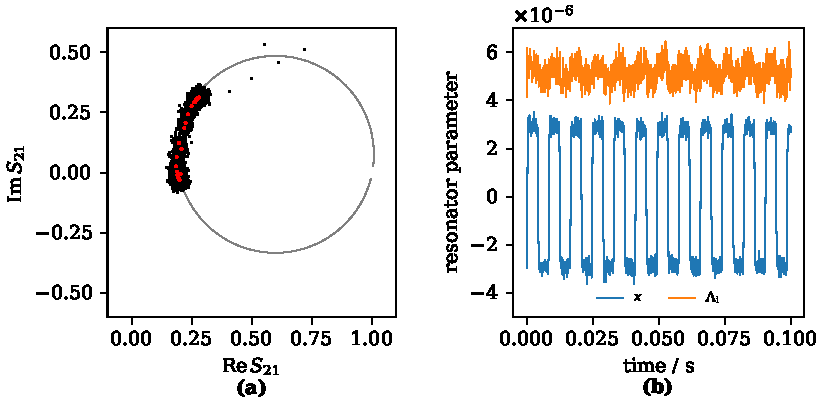
\includegraphics[width=\textwidth]{theory/example_time-ordered_data.pdf}
\caption
[Time-ordered data showing the response to millimeter-wave light.]
{Time-ordered data showing the response to millimeter-wave light.
The device is an aluminum lumped-element KID that was used for the published research described in Chapter~\ref{chp:sensitivity}.
The output of the millimeter-wave source was chopped at \SI{122}{Hz}.
The entire time series is about \SI{4}{s} and is sampled at \SI{31}{kHz}.
\textbf{(a)}
The real and imaginary parts of $\forwardscattering$.
The gray line is the resonator model, the small black points are all the data, and the red points are calculated by averaging all points separated by one period of the signal used to chop the source.
The few points that are widely separated from the rest, to the upper right, were probably caused by a cosmic ray impact.
\textbf{(b)}
The time-varying resonator parameters versus time.
Only \SI{0.1}{s} of data is shown.
The detuning response is much larger than the loss response, as expected for a device with such a low resonance frequency.
}
\label{fig:example_time-ordered_data}
\end{figure}
